\begin{figure}[tbp]
\centering
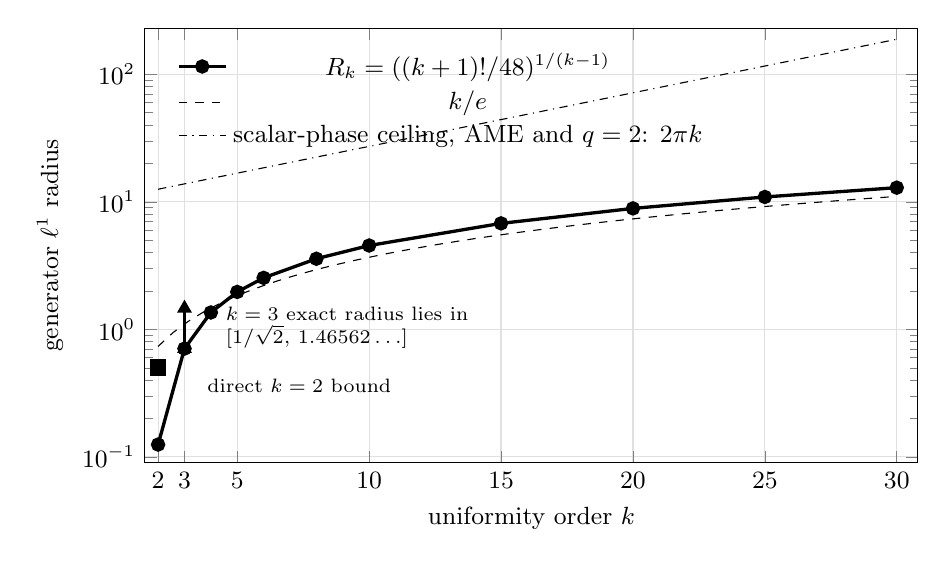
\begin{tikzpicture}
\begin{axis}[
  width=0.94\textwidth,
  height=7.1cm,
  xlabel={uniformity order $k$},
  ylabel={generator $\ell^1$ radius},
  xmin=1.5,xmax=30.8,
  ymin=0.09,ymax=230,
  ymode=log,
  log basis y=10,
  xtick={2,3,5,10,15,20,25,30},
  grid=major,
  grid style={black!12},
  legend style={draw=none,fill=none,font=\small,at={(0.03,0.97)},anchor=north west},
  tick label style={font=\small},
  label style={font=\small}
]
  \addplot[black,very thick,mark=*] coordinates {
    (2,0.125000) (3,0.707107) (4,1.357209) (5,1.967990)
    (6,2.536517) (8,3.581579) (10,4.547454) (15,6.782412)
    (20,8.887812) (25,10.927372) (30,12.927355)
  };
  \addlegendentry{$R_k=((k+1)!/48)^{1/(k-1)}$}
  \addplot[black,dashed,domain=2:30,samples=50] {x/2.718281828};
  \addlegendentry{$k/e$}
  \addplot[black,dashdotted,domain=2:30,samples=2] {2*pi*x};
  \addlegendentry{scalar-phase ceiling, AME and $q=2$: $2\pi k$}

  \addplot[only marks,mark=square*,mark size=2.8pt,black]
    coordinates {(2,0.5)};
  \node[anchor=west,font=\scriptsize] at (axis cs:3.5,0.36)
    {direct $k=2$ bound};

  \addplot[black,very thick] coordinates {(3,0.707107) (3,1.46562)};
  \addplot[only marks,mark=triangle*,mark size=2.7pt,black]
    coordinates {(3,0.707107) (3,1.46562)};
  \node[anchor=west,align=left,font=\scriptsize] at (axis cs:4.2,1.03)
    {$k=3$ exact radius lies in\\$[1/\sqrt2,\,1.46562\ldots]$};
\end{axis}
\end{tikzpicture}
\caption{Certified generator \(\ell^1\) radius of the quadratic stability
estimate against uniformity order.  The general radius
\(R_k=((k+1)!/48)^{1/(k-1)}\) grows as \(k/e\); scalar-phase configurations
bound every such radius by \(2\pi(1-1/q)n\), so linear growth is the maximal
order.  For an \(\AME(2m,q)\) state, \(k=m\).  At \(k=3\), the
Reed--Muller family pins the exact radius for the constant
\(\sqrt{6q/5}\) inside the displayed interval.}
\label{fig:stability-radius}
\end{figure}
